\documentclass{article}
\usepackage[a4paper,margin=1in]{geometry}
\usepackage{titlesec}
\usepackage{hyperref}
\usepackage{graphicx}

\title{\textbf{Testing the Alcohol Detection System in Real-World Conditions}}
\author{}
\date{}
%source available on github.com/abhinavdatta
\begin{document}
\maketitle

\section{Understanding the Problem of Drunk Driving on Bikes}
\begin{figure}[h!]
    \centering
    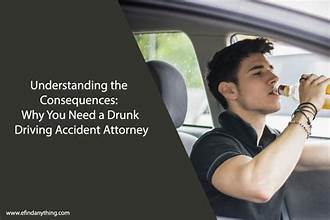
\includegraphics[width=0.6\textwidth]{ac/1.jpg}
    \caption{Person drinking and driving}
    \label{fig:Drinking_water}
\end{figure}

\subsection{Problem Identification -- High Accident Rates Due to Drunk Driving}
\begin{itemize}
    \item \textbf{Data-Driven Insight}: Statistics on bike accidents involving alcohol (e.g., \% of fatalities linked to drunk riding).
    \item \textbf{Legal Gaps}: Weak enforcement for bikes vs. cars in many regions.
    \item \textbf{Behavioral Factors}: Riders underestimating impairment risks compared to car drivers.
\end{itemize}

\subsection{User Research -- Challenges in Detecting Alcohol Consumption Before Driving}
\begin{itemize}
    \item \textbf{Interviews/Surveys}: Riders admit to ignoring sobriety checks due to convenience.
    \item \textbf{Observation}: No standardized pre-ride alcohol tests for bikes (unlike car ignition interlocks).
    \item \textbf{Psychological Barriers}: Peer pressure, overconfidence in riding ability while intoxicated.
\end{itemize}

\subsection{Competitor Analysis -- Existing Alcohol Detection Systems in Cars}
\begin{itemize}
    \item \textbf{Technologies Reviewed}: Breathalyzer ignition interlocks, touch-based sensors (e.g., steering wheel), AI-powered cameras (detecting drowsiness).
    \item \textbf{Gaps for Bikes}: Car systems are bulky/power-intensive; bikes need lightweight, portable solutions.
\end{itemize}

\subsection{Safety Concerns -- Risk to Rider, Passenger, and Public}
\begin{itemize}
    \item \textbf{Multi-Party Impact}: Collisions with pedestrians, vehicles, or fixed objects.
    \item \textbf{Secondary Risks}: Head injuries (low helmet usage among drunk riders).
\end{itemize}

\subsection{Pain Points Summary}
\begin{itemize}
    \item \textbf{Lack of Enforcement}: No legal mandate for bike alcohol detection.
    \item \textbf{Slow Reaction Time}: Current sensors take 5+ seconds (unideal for bikes).
    \item \textbf{False Negatives}: Sensors fail in cold/humid conditions or with mouthwash.
\end{itemize}

\newpage

\section{Defining the Need for a Bike-Integrated Alcohol Detection System}
\begin{figure}[h!]
    \centering
    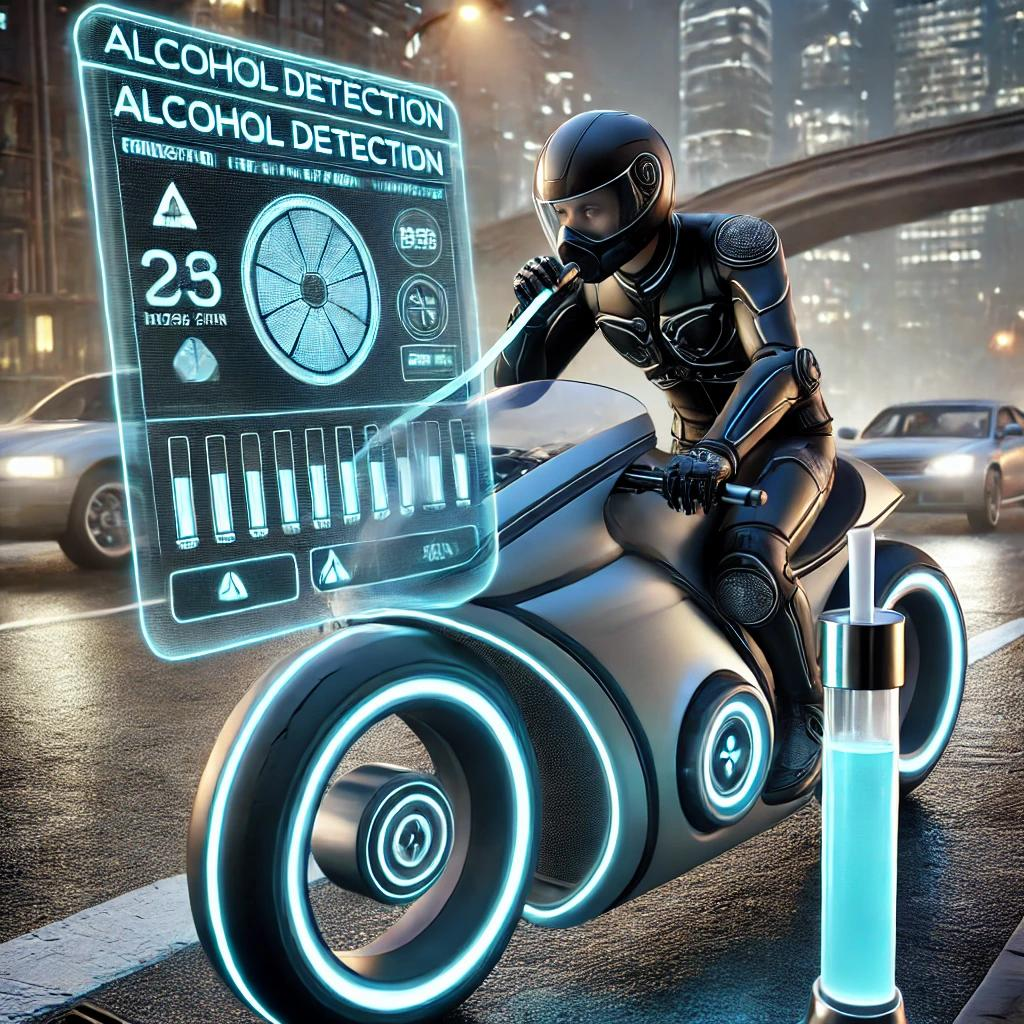
\includegraphics[width=0.6\textwidth]{2.1.jpg}
    \caption{Person drinking from filter straw}
    \label{fig:Drinking_water}
\end{figure}

\subsection{Define the Problem Statement -- How Might We Prevent Drunk Driving on Bikes?}
\begin{itemize}
    \item \textbf{Reframed as a Design Challenge}:
    \begin{quote}
        ``Design a non-intrusive, bike-compatible system that detects alcohol levels in real-time, prevents ignition if impaired, and alerts authorities if tampered with.''
    \end{quote}
\end{itemize}

\subsection{User Persona and Pain Points -- Daily Commuters, Young Riders, and Law Enforcement}
\begin{itemize}
    \item \textbf{Daily Commuters}: Need quick, seamless checks (e.g., handlebar-mounted sensor).
    \item \textbf{Young Riders}: High-risk group; may resist "nanny" tech $\rightarrow$ gamify sobriety checks?
    \item \textbf{Law Enforcement}: Needs tamper-proof data for legal evidence.
\end{itemize}

\subsection{Scope of the Problem -- Urban, Rural, and Highway Scenarios}
\begin{itemize}
    \item \textbf{Urban}: Frequent stops $\rightarrow$ quick retests.
    \item \textbf{Rural}: Poor connectivity $\rightarrow$ offline functionality.
    \item \textbf{Highway}: High speed $\rightarrow$ fail-safe shutdown (e.g., gradual speed reduction).
\end{itemize}

\subsection{Success Criteria -- Fast, Accurate, and Tamper-Proof Detection}
\begin{itemize}
    \item \textbf{Accuracy}: $<0.01\%$ false positives (calibrated to legal BAC limits).
    \item \textbf{Speed}: Detection in $<3$ seconds.
    \item \textbf{Tamper-Proof}: GPS alerts if bike is moved after failed test.
\end{itemize}

\subsection{Design Constraints -- Sensor Size, Power Consumption, and Weather Resistance}
\begin{itemize}
    \item \textbf{Sensor Size}: Must fit on handlebars/helmet without impeding ride.
    \item \textbf{Power}: Solar/bike dynamo-powered to avoid battery swaps.
    \item \textbf{Weather Resistance}: Operates in rain ($-10^\circ$C to $50^\circ$C range).
\end{itemize}

\newpage

% ==========================
% SECTION 3: GENERATING IDEAS
% ==========================
\section{Generating Ideas for an Alcohol Detection System}



\subsection{Brainstorming Ideas -- Breathalyzer, Fingerprint-Based Detection, and Eye-Tracking}
\begin{itemize}
    \item \textbf{Breathalyzer}: Traditional approach; requires rider exhalation into a handlebar-mounted sensor.
    \item \textbf{Fingerprint-Based Detection}: Measures alcohol secretion through sweat (e.g., electrochemical skin sensors).
    \item \textbf{Eye-Tracking}: Uses mini-cameras to detect pupil dilation/nystagmus (limited accuracy in low light).
\end{itemize}

\subsection{Concept Selection -- Choosing the Most Practical and Reliable Solution}
\begin{itemize}
    \item \textbf{Evaluation Criteria}: Cost, power efficiency, and rider compliance.
    \item \textbf{Shortlist}: Hybrid breathalyzer + skin sensor for redundancy.
\end{itemize}

\subsection{Mind Mapping -- Linking Detection, Engine Lock, and Rider Safety}
\begin{itemize}
    \item \textbf{System Flow}: 
    \begin{itemize}
        \item Detection $\rightarrow$ BAC analysis $\rightarrow$ Engine lock (if BAC $>0.05\%$) $\rightarrow$ GPS alert to authorities.
    \end{itemize}
    \item \textbf{Fail-Safes}: Manual override for emergencies (e.g., hospital trips).
\end{itemize}

\subsection{Sketching Initial Designs -- Sensor Placement on Handlebar or Helmet}
\begin{itemize}
    \item \textbf{Handlebar}: Proximity to rider’s mouth (breathalyzer); risk of weather damage.
    \item \textbf{Helmet}: Non-intrusive but requires wireless link to bike’s ignition.
\end{itemize}

\subsection{Prioritizing Ideas -- Balancing Accuracy, Response Time, and User Comfort}
\begin{itemize}
    \item \textbf{Top Priority}: Sub-3-second response time (to match bike ignition sequences).
    \item \textbf{Trade-offs}: Smaller sensors may sacrifice accuracy; require calibration.
\end{itemize}

\newpage

% ================================
% SECTION 4: DEVELOPING PROTOTYPES
% ================================
\section{Developing and Prototyping the Alcohol Detection System}

\begin{figure}[h!]
    \centering
    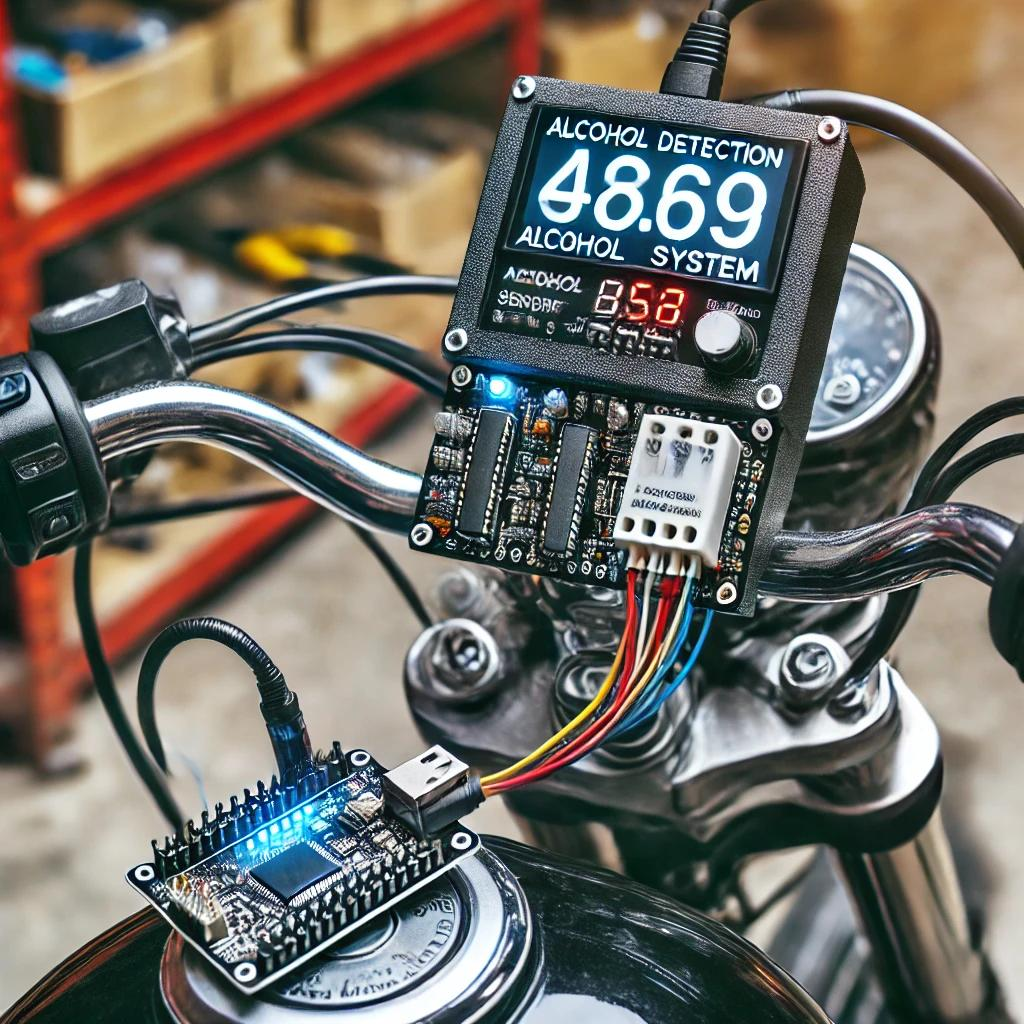
\includegraphics[width=0.6\textwidth]{4.jpg}
    \caption{Person drinking from filter straw}
    \label{fig:Drinking_water}
\end{figure}


\subsection{Prototype Development -- Creating Sensor and Locking Mechanism Models}
\begin{itemize}
    \item \textbf{Modular Design}: 3D-printed sensor housing with Arduino/Raspberry Pi for testing.
    \item \textbf{Locking Mechanism}: Solenoid-based bike ignition lock (compatible with e-bikes).
\end{itemize}

\subsection{Sensor Type Testing -- Breathalyzer vs Skin-Based Alcohol Sensors}
\begin{itemize}
    \item \textbf{Breathalyzer}: 
    \begin{itemize}
        \item Pros: High accuracy (FDA-approved for cars).
        \item Cons: Requires rider cooperation (exhalation).
    \end{itemize}
    \item \textbf{Skin Sensors}: 
    \begin{itemize}
        \item Pros: Passive detection (e.g., via handlebar grips).
        \item Cons: Slower response in cold weather.
    \end{itemize}
\end{itemize}

\subsection{Connectivity Testing -- Linking Sensor to Ignition and Mobile Alerts}
\begin{itemize}
    \item \textbf{Wired vs Wireless}: Bluetooth Low Energy (BLE) for helmet-mounted sensors; wired for handlebar.
    \item \textbf{Mobile Integration}: Alert riders via vibration/phone notification before engine lock.
\end{itemize}

\subsection{Feasibility Testing -- Ensuring Quick and Reliable Detection}
\begin{itemize}
    \item \textbf{Lab Tests}: Simulated drunk riding (alcohol spray in controlled environments).
    \item \textbf{Field Tests}: Real-world scenarios (e.g., rain, vibrations).
\end{itemize}

\subsection{Design Adjustments -- Improving Sensor Response Time and Accuracy}
\begin{itemize}
    \item \textbf{Calibration}: Auto-calibration using environmental data (temperature/humidity).
    \item \textbf{Feedback Loop}: Rider-facing LED indicators for system status (green/red lights).
\end{itemize}

\newpage

\section {5.Testing the Alcohol Detection System in Real-World Conditions}

\begin{figure}[h!]
    \centering
    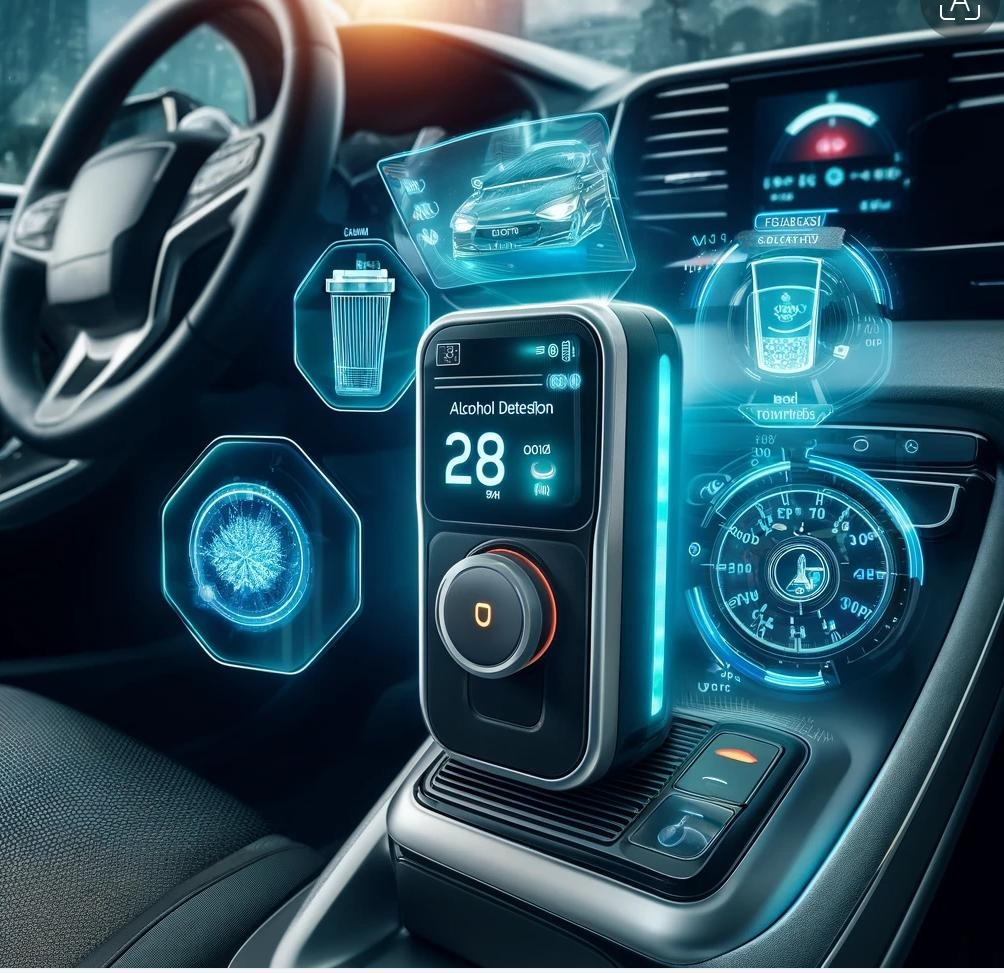
\includegraphics[width=0.6\textwidth]{ac/5.jpg}
    \caption{Person drinking from filter straw}
    \label{fig:Drinking_water}
\end{figure}


\subsection {5.1 Environmental Testing – Different Temperatures, Humidity, and Dust Conditions}
The alcohol detection system must function accurately in various environmental conditions. This involves testing the sensor's performance under extreme temperatures (hot and cold), high and low humidity levels, and exposure to dust. This ensures the system maintains reliability regardless of weather or geographic location.

Additional considerations:
\begin{itemize}
    \item \textbf{Water and Moisture Resistance}: Ensuring sensors function in wet conditions such as rain or accidental liquid spills.
    \item \textbf{Electromagnetic Interference}: Testing against interference from electronic devices and vehicle components.
    \item \textbf{Altitude and Air Pressure Variations}: Verifying performance at different elevations where air composition changes.
\end{itemize}

\subsection {5.2 Feedback Analysis – From Riders and Law Enforcement}
Gathering feedback from vehicle users and law enforcement helps assess the system’s practicality. Riders can provide insights into ease of use, response time, and potential inconveniences, while law enforcement can evaluate its effectiveness in reducing alcohol-related accidents. This feedback is crucial for refining the system.

Additional considerations:
\begin{itemize}
    \item \textbf{User-Friendly Interface}: Ensuring intuitive operation and minimal disruption to the driver.
    \item \textbf{Cultural and Regional Acceptance}: Evaluating societal acceptance of the technology.
    \item \textbf{Integration with Smart Devices}: Feedback on smartphone connectivity and app integration.
\end{itemize}

\subsection {5.3 Iterative Improvements – Adjusting Sensitivity and False Positive Rates}
To enhance accuracy, the system must be fine-tuned to minimize false positives (detecting alcohol when none is present) and false negatives (failing to detect alcohol). This involves adjusting sensitivity thresholds, improving sensor algorithms, and optimizing software to reduce errors while ensuring user safety.

Additional considerations:
\begin{itemize}
    \item \textbf{Machine Learning Algorithms}: Implementing AI-driven models to improve accuracy over time.
    \item \textbf{Real-Time Updates}: Enabling software updates for performance improvements.
    \item \textbf{Cross-Verification with Multiple Sensors}: Using redundant sensors to confirm alcohol detection.
\end{itemize}

\subsection {5.4 Safety Testing – Ensuring No Ignition Failure or Accidental Locking}
The system must undergo rigorous testing to prevent malfunctions such as accidental vehicle lockout or failure to start due to sensor errors. This includes redundancy checks, fail-safe mechanisms, and backup procedures to ensure that the vehicle remains operational under normal conditions while effectively restricting drunk driving.

Additional considerations:
\begin{itemize}
    \item \textbf{Emergency Override Mechanism}: Allowing emergency personnel to bypass the system.
    \item \textbf{Long-Term Durability}: Evaluating wear and tear on sensors over extended use.
    \item \textbf{Backup Power Supply}: Ensuring the system functions even if the vehicle's battery is low.
\end{itemize}

\subsection{Final Validation – Meeting Automotive and Safety Standards}
Before deployment, the system must comply with industry regulations such as ISO (International Organization for Standardization) and NHTSA (National Highway Traffic Safety Administration) guidelines. Final validation involves certification tests, regulatory approvals, and compliance with safety standards to ensure legal and market readiness.

Additional considerations:
\begin{itemize}
    \item \textbf{Crash and Impact Testing}: Verifying system integrity during vehicle accidents.
    \item \textbf{Compliance with Data Privacy Laws}: Ensuring collected data is secure and used responsibly.
    \item \textbf{Scalability and Cost Efficiency}: Evaluating mass production feasibility and affordability.
\end{itemize}

\newpage

% ==============================================
% SECTION 6: MANUFACTURING A RELIABLE SYSTEM
% ==============================================
\section{Manufacturing a Reliable and Tamper-Proof Alcohol Detection System}

\begin{figure}[h!]
    \centering
    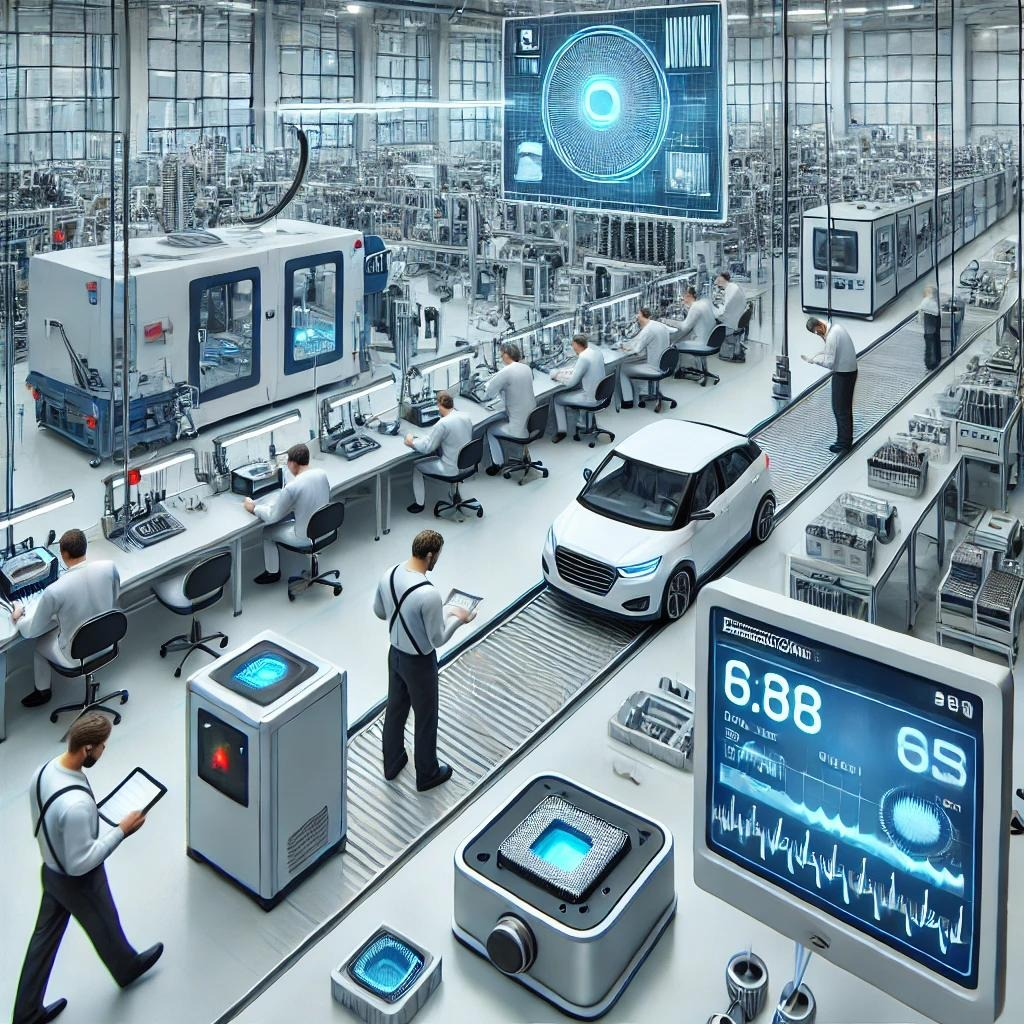
\includegraphics[width=0.6\textwidth]{ac/6.jpg}
    \caption{Person drinking from filter straw}
    \label{fig:Drinking_water}
\end{figure}

\subsection{Final Product Design -- Optimizing for Size, Power Usage, and Efficiency}
\begin{itemize}
    \item \textbf{Compact Design}: Integrated sensor module (size: $5 \times 3 \times 2$ cm) mounted on handlebars or helmet.
    \item \textbf{Power Efficiency}: Uses rechargeable Li-ion battery with solar assist (5-day standby time).
    \item \textbf{Tamper-Proofing}: Epoxy-sealed circuitry and GPS tracking if disassembled.
\end{itemize}

\subsection{Manufacturing Considerations -- Material Sourcing and Sensor Calibration}
\begin{itemize}
    \item \textbf{Materials}:
    \begin{itemize}
        \item Housing: Weatherproof polycarbonate (IP67 rating).
        \item Sensors: MEMS-based ethanol detectors (sourced from automotive suppliers).
    \end{itemize}
    \item \textbf{Calibration}: Factory pre-calibration with quarterly software updates.
\end{itemize}

\subsection{Quality Control -- Ensuring Consistent Sensor Performance}
\begin{itemize}
    \item \textbf{Testing Protocols}:
    \begin{itemize}
        \item Batch testing for false positives/negatives (99.9\% accuracy target).
        \item Vibration/shock tests (simulating rough terrain).
    \end{itemize}
    \item \textbf{Compliance}: Meets ISO 26262 (functional safety) and FCC/CE standards.
\end{itemize}

\subsection{Cost Analysis -- Balancing Production Costs and Affordability}
\begin{itemize}
    \item \textbf{BOM Cost}: \$18/unit at scale (10,000 units), retail target: \$49.
    \item \textbf{Trade-offs}: Cheaper skin sensors vs. higher-accuracy breathalyzers (+\$7/unit).
\end{itemize}

\subsection{Production Timeline -- Planning for Mass Production and Distribution}
\begin{itemize}
    \item \textbf{Phases}:
    \begin{itemize}
        \item Pilot batch (500 units): 3 months (testing/feedback).
        \item Full production: 12 months (scaling to 50,000 units/year).
    \end{itemize}
    \item \textbf{Distribution}: Partner with bike manufacturers (OEM) and aftermarket retailers.
\end{itemize}

\newpage

% ==============================================
% SECTION 7: ENHANCING USER EXPERIENCE AND SAFETY
% ==============================================
\section{Enhancing User Experience and Safety Mechanisms}

\begin{figure}[h!]
    \centering
    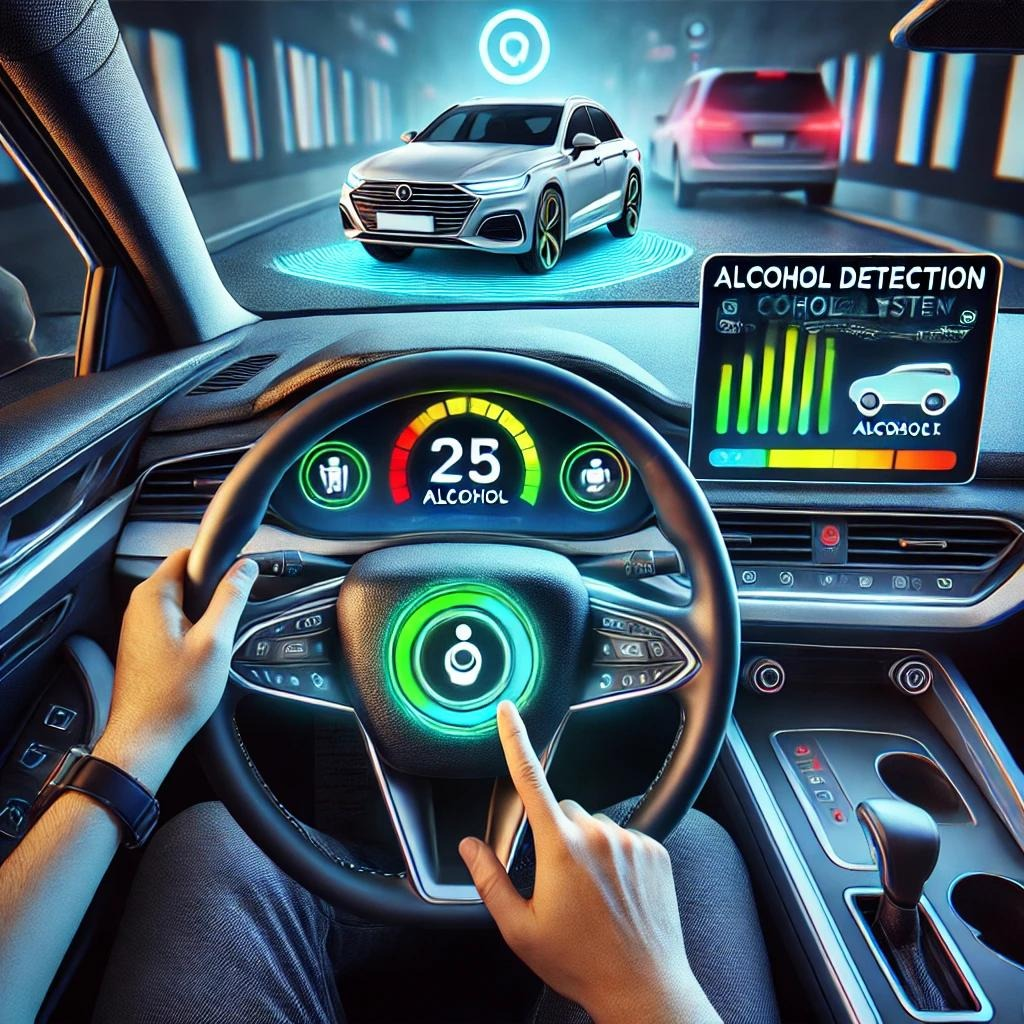
\includegraphics[width=0.6\textwidth]{ac/7.jpg}
    \caption{Person drinking from filter straw}
    \label{fig:Drinking_water}
\end{figure}

\subsection{Usability Testing -- Ease of Installation and Rider Interaction}
\begin{itemize}
    \item \textbf{Installation}: Tool-free clip-on design (compatible with 90\% of bike models).
    \item \textbf{Interaction}: Single-button operation with voice feedback ("Blow to start").
\end{itemize}

\subsection{Rider Notification -- Visual and Audio Alerts for Detection Status}
\begin{itemize}
    \item \textbf{Visual}: RGB LED (Green = sober, Red = impaired, Blue = system error).
    \item \textbf{Audio}: Gradual escalation (beep $\rightarrow$ voice warning $\rightarrow$ siren if tampering detected).
\end{itemize}

\subsection{Emergency Override -- Allowing Emergency Unlock in Case of System Failure}
\begin{itemize}
    \item \textbf{Mechanism}: Physical key override (hidden compartment) + PIN via mobile app.
    \item \textbf{Logging}: Records all overrides with timestamp/GPS for liability.
\end{itemize}

\subsection{Design Adjustments Based on UX -- Improving Comfort and Sensor Placement}
\begin{itemize}
    \item \textbf{Ergonomics}: Curved handlebar mount to avoid wrist contact.
    \item \textbf{Helmet Version}: Reduced weight ($<50$g) with airflow vents to prevent overheating.
\end{itemize}

\subsection{Emotional Impact -- Building Confidence and Promoting Safe Riding}
\begin{itemize}
    \item \textbf{Gamification}: Mobile app rewards sober rides with discounts on maintenance.
    \item \textbf{Community}: Share anonymized safe-riding stats to foster peer accountability.
\end{itemize}

\newpage

% ==============================================
% SECTION 8: SUSTAINABILITY AND LONG-TERM PERFORMANCE
% ==============================================
\section{Ensuring Sustainability and Long-Term Performance}
\begin{figure}[h!]
    \centering
    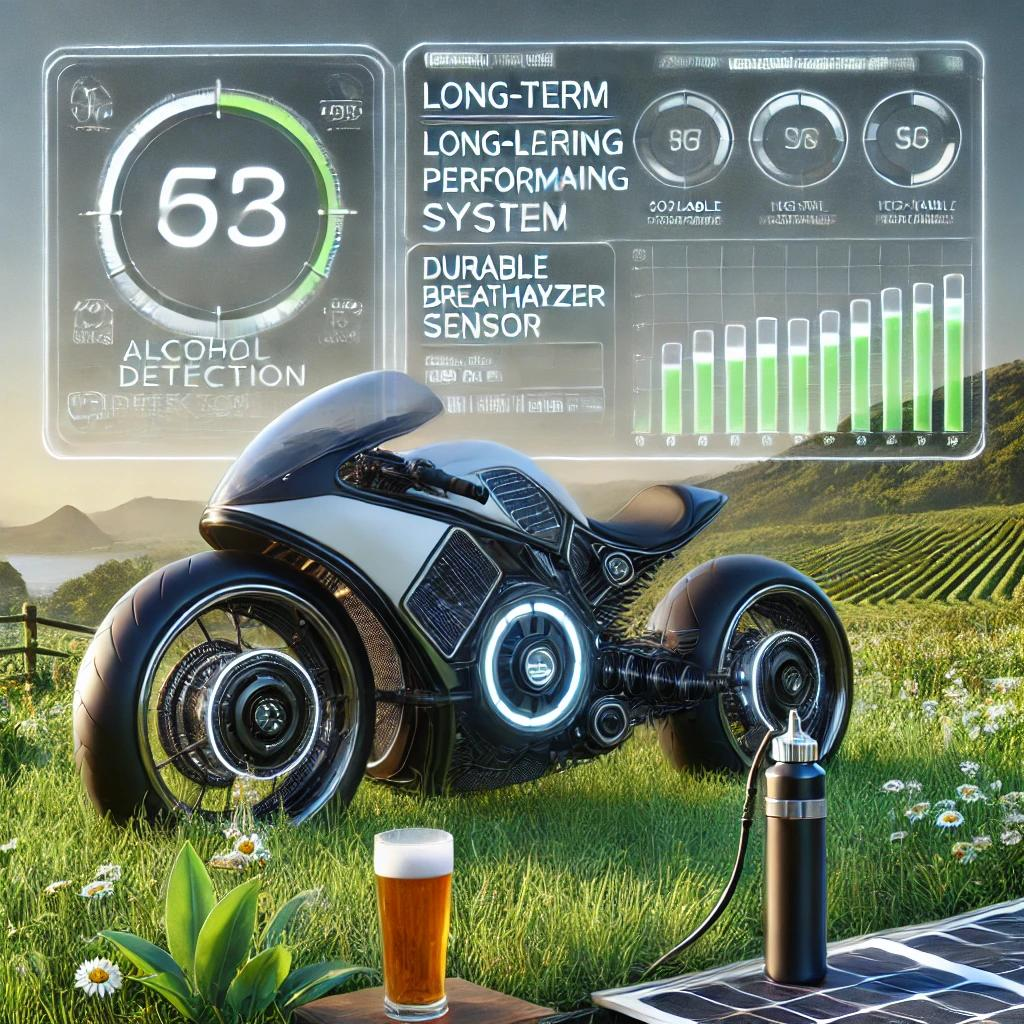
\includegraphics[width=0.6\textwidth]{ac/8.jpg}
    \caption{Person drinking from filter straw}
    \label{fig:Drinking_water}
\end{figure}
\subsection{Material Sourcing -- Using Eco-Friendly and Recyclable Materials}
\begin{itemize}
    \item \textbf{Housing Material}: Recycled polycarbonate (70\% post-consumer waste) with biodegradable padding.
    \item \textbf{Electronics}: Lead-free solder and conflict-free minerals in PCB manufacturing.
    \item \textbf{Supplier Criteria}: ISO 14001-certified partners for reduced carbon footprint.
\end{itemize}

\subsection{Environmental Impact -- Minimizing Power Consumption}
\begin{itemize}
    \item \textbf{Low-Power Design}: Sleep mode (0.1W) when idle, 1.2W during active detection.
    \item \textbf{Renewable Options}: Solar panel add-on (2W) for self-charging in daylight.
    \item \textbf{Energy Recovery}: Regenerative braking integration for e-bikes.
\end{itemize}

\subsection{Longevity Testing -- Ensuring Accuracy Over Long-Term Use}
\begin{itemize}
    \item \textbf{Accelerated Aging}: Simulated 5-year use in extreme conditions (-20°C to 60°C).
    \item \textbf{Sensor Drift Mitigation}: Auto-calibration every 100 uses or 30 days.
    \item \textbf{Component Lifespan}: Replaceable sensor heads (rated for 50,000 tests).
\end{itemize}

\subsection{Maintenance -- Easy Replacement of Sensors and Calibration}
\begin{itemize}
    \item \textbf{Modular Design}: Tool-free sensor cartridge replacement (30-second swap).
    \item \textbf{User Calibration}: Guided process via mobile app with QR code verification.
    \item \textbf{Service Network}: Partnered bike shops for free annual check-ups.
\end{itemize}

\subsection{Disposal Guidelines -- Safe and Eco-Friendly Disposal Options}
\begin{itemize}
    \item \textbf{Recycling Program}: Pre-paid return mailer for battery/sensor recycling.
    \item \textbf{Hazardous Materials}: Separate disposal instructions for Li-ion batteries.
    \item \textbf{End-of-Life}: 85\% component recyclability rate (certified by e-Stewards).
\end{itemize}


\newpage

% ==============================================
% SECTION 9: MARKET POSITIONING
% ==============================================
\section{Positioning the Alcohol Detection System in the Market}

\subsection{Market Positioning -- Highlighting Safety and Prevention Benefits}
\begin{itemize}
    \item \textbf{Key Message}: "The Guardian Angel for Night Riders" – focus on accident reduction stats.
    \item \textbf{USP}: Only bike-specific system with tamper-proof GPS alerts.
    \item \textbf{Price Tier}: Mid-range (\$49) – positioned as "insurance" against DUI fines (\$500+).
\end{itemize}

\subsection{Brand Identity -- Promoting Responsible Riding and Accident Prevention}
\begin{itemize}
    \item \textbf{Visual Identity}: Shield logo with green/black color scheme (safety + tech).
    \item \textbf{Tone}: Empowering ("Take Control") not punitive ("Big Brother").
    \item \textbf{Campaigns}: #SoberPedals social media challenge with influencer riders.
\end{itemize}

\subsection{Packaging Design -- Compact and Informative Packaging}
\begin{itemize}
    \item \textbf{Eco-Packaging}: Mushroom-based foam inserts, soy ink printed manuals.
    \item \textbf{Quick Start}: Pictogram-based setup guide (no text needed).
    \item \textbf{Regulatory}: DOT/CE markings prominently displayed.
\end{itemize}

\subsection{Target Audience Analysis -- Riders, Bike Manufacturers, and Safety Regulators}
\begin{itemize}
    \item \textbf{Primary}:
    \begin{itemize}
        \item \textbf{E-Bike Commuters}: Urban riders (age 18-35) with \geq \$500 bikes.
        \item \textbf{Bike-Sharing Companies}: Fleet safety compliance.
    \end{itemize}
    \item \textbf{Secondary}:
    \begin{itemize}
        \item \textbf{Insurers}: Discounts for bikes with installed systems.
        \item \textbf{Governments}: Subsidy programs for high-risk areas.
    \end{itemize}
\end{itemize}

\subsection{Promotion Strategy -- Partnering With Bike Brands, Traffic Police, and Safety Campaigns}
\begin{itemize}
    \item \textbf{OEM Partnerships}: Bundled with premium bikes (e.g., Specialized, Trek).
    \item \textbf{Law Enforcement}: Pilot programs with traffic police (data sharing opt-in).
    \item \textbf{Events}: Demo booths at bike expos and DUI checkpoints.
\end{itemize}

\newpage

% ==============================================
% SECTION 10: POST-LAUNCH REVIEW AND IMPROVEMENT
% ==============================================
\section{Post-Launch Review and Continuous Improvement}

\subsection{Customer Feedback Collection -- From Riders and Safety Agencies}
\begin{itemize}
    \item \textbf{Multi-Channel Input}:
    \begin{itemize}
        \item In-app surveys (5-second pulse checks after each ride)
        \item Focus groups with traffic police and bike-sharing operators
        \item Social media sentiment analysis (\#BikeSober trends)
    \end{itemize}
    \item \textbf{Key Metrics}: Net Promoter Score (NPS) target $\geq 65$
\end{itemize}

\subsection{Performance Review -- Sensor Accuracy and False Detection Rate}
\begin{itemize}
    \item \textbf{Field Data Analysis}:
    \begin{itemize}
        \item Monthly false positive rate (goal: $<0.1\%$)
        \item Weather-related failures (rain/humidity correlation)
    \end{itemize}
    \item \textbf{Benchmarking}: Compare against car ignition interlocks (NHTSA standards)
\end{itemize}

\subsection{Version Updates -- Improving Detection Speed and Weather Resistance}
\begin{itemize}
    \item \textbf{Firmware Updates}:
    \begin{itemize}
        \item Over-the-air (OTA) updates every 3 months
        \item Adaptive algorithms for tropical vs. arid climates
    \end{itemize}
    \item \textbf{Hardware Revisions}: 
    \begin{itemize}
        \item Gen 2: Graphene-coated sensors (2025 Q3)
        \item Gen 3: Self-heating elements for sub-zero temps (2026)
    \end{itemize}
\end{itemize}

\subsection{Customer Support Strategy -- Handling Maintenance and Repairs}
\begin{itemize}
    \item \textbf{Tiered Support}:
    \begin{itemize}
        \item Level 1: Chatbot troubleshooting (80\% resolution)
        \item Level 2: Video call technicians (15-min response time)
        \item Level 3: On-site service for fleet operators
    \end{itemize}
    \item \textbf{Warranty}: 2-year comprehensive coverage + crash replacement discounts
\end{itemize}

\subsection{Future Enhancements -- AI-Based Detection, Fatigue Monitoring, and Helmet Integration}
\begin{itemize}
    \item \textbf{AI Roadmap}:
    \begin{itemize}
        \item Voice slur detection via helmet mic (patent pending)
        \item Pupil tracking with $10 \times 10$mm IR cameras
    \end{itemize}
    \item \textbf{Cross-Platform}:
    \begin{itemize}
        \item Integration with smart helmets (e.g., Livall, Sena)
        \item Sync with fitness trackers for fatigue alerts
    \end{itemize}
    \item \textbf{Regulatory}: Preparing for EU \& US bike safety mandates (2027+)
\end{itemize}

\end{document}
